\section{Bispace Propagation Model}

\begin{figure}[ht]
\centering
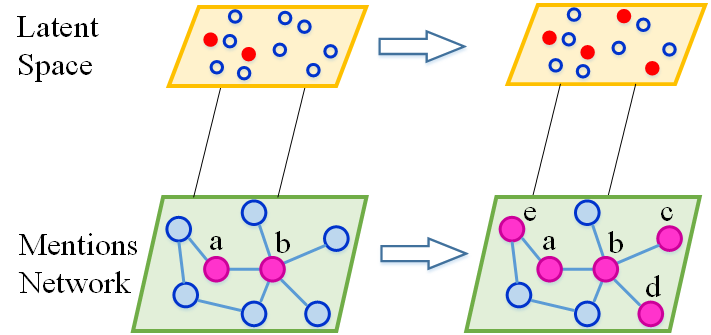
\includegraphics[width=3.5in] {figures/Bio-space.png}
\caption{Bispace propagation model. In the latent space, users infections are explained by a Poisson model, and the red nodes denote the infected users from one time step to another. In the mentions network space, users are infected according to the GBM model. Here, the purple nodes (a, b, c, d, e) denote user infections explained by the GBM model. }
\label{fig:bi-space}
\end{figure}


Many information diffusion models assume that propagation occurs over a single domain.
However, it is hard to build a complete, exhaustive network of interactions.
For instance, consider building a network based only on which Twitter users follow which other users. This network will miss interactions such as retweets and mentions and the effect of influences originating
outside of Twitter. Therefore, considering only a single space will make it difficult to account for all possible factors that influence the spread of information.
In this study, we propose a bispace diffusion model that accounts for two domains of diffusion: the observed social network and the latent space, as can be seen in Fig.~\ref{fig:bi-space}.
In our case, the observed user space is the Twitter mentions network,
whereas the latent space refers to any interactions outside of this network.
To account for varying diffusion dynamics, each space is intended to have
its own propagation model.
As described earlier, we model propagation through the Twitters mentions network as Geometric Brownian motion. We use the Poisson distribution to describe information propagation in the latent space.

\subsection{GBM with Communities}
\begin{figure}[t]
\centering
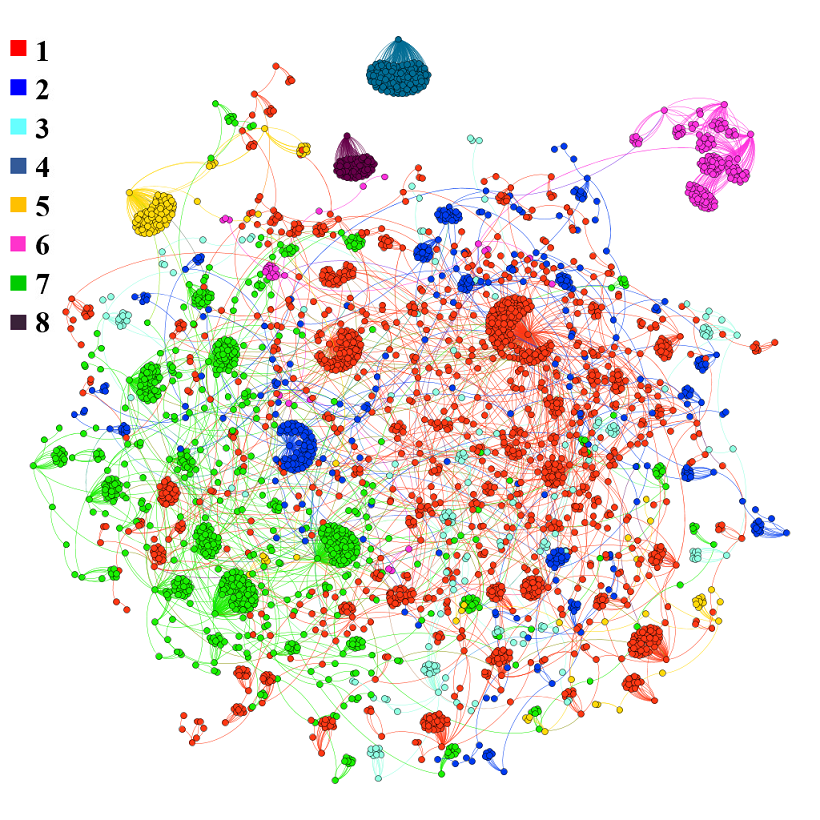
\includegraphics[width=3.5in] {figures/4_teacher_major_community.png}
\caption{Major communities of teacher protest events (Sept 1 to Sept 12, 2013,
Mexico).}
\label{fig:teacher_major_community}
\end{figure}


\begin{figure}[t]
\centering
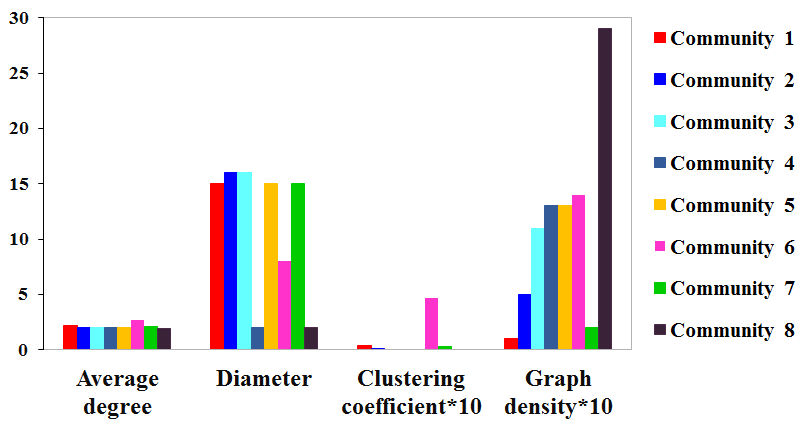
\includegraphics[width=4in] {figures/4teacher-community-parameters.png}
\caption{Key graph properties of communities underlying the Mexican teacher protest events.}
\label{fig:teacher_community_parameters0}
\end{figure}

Within networks, a community refers to the appearance of densely connected groups of vertices, with sparse connections between each group~\cite{newman2006modularity}.
Instead of treating the whole network as a single propagation space,
we use network structure to further split the network into communities.
For our mentions network we use the Louvain method~\cite{blondel2008fast} for community detection to split the network into groups of users. For each community of users we can calculate classical graph features such as average degree, diameter, density, and clustering coefficient with which we can characterize them. In Fig.~\ref{fig:teacher_community_parameters0} we plot several features for each of the 8 communities found in the case study of Mexican teachers protest of 2013. Diameter $r = \max dist(v_i, v_j)$ is the length (in number of edges) of the longest geodesic path between any nodes $v_i$ and $v_j$~\cite{newman2003structure}. The clustering coefficient $c_i$ is the proportion of node $v_i$'s neighbors that are connected. Graph density is defined as $\frac{2|E|}{|V|(|V|-1)}$ where $E$ is the number of edges and $V$ is the
number of nodes~\cite{scott2011sage}. As shown in Fig.~\ref{fig:teacher_community_parameters0}, diameter and graph density vary considerably.


\begin{figure}[t]
\centering
\subfigure[Raw data]{
   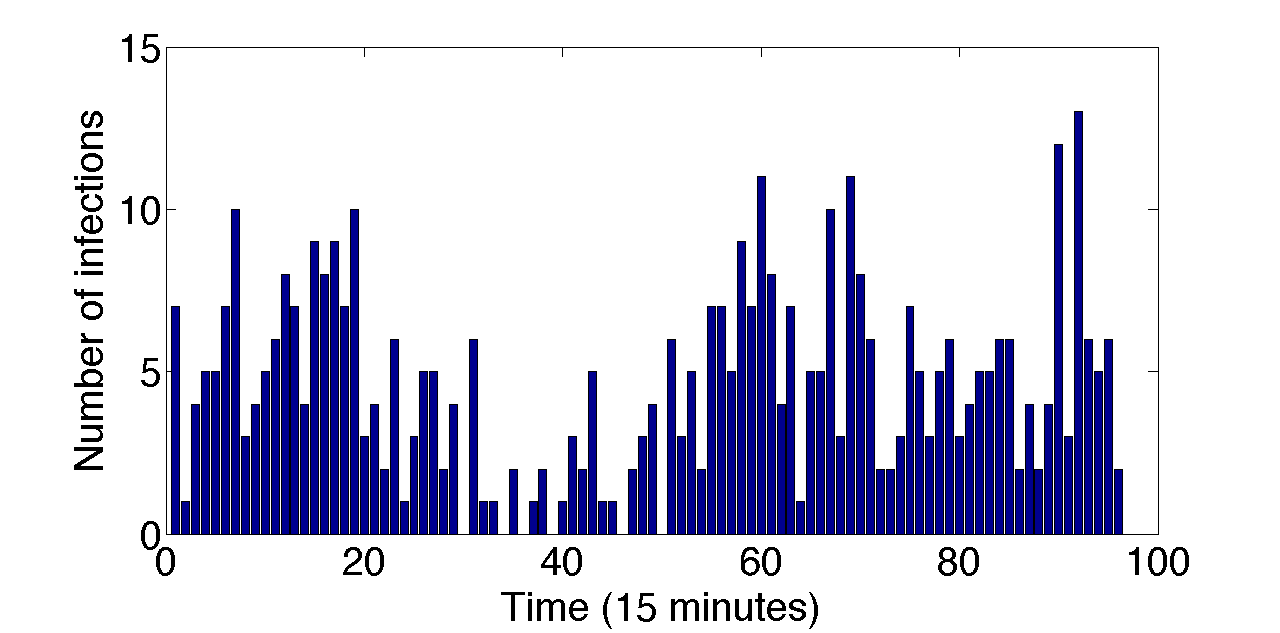
\includegraphics[width=3in,height=1.5in] {figures/Poisson_realData.png}
  \label{fig:Poisson_Sep3}
 }
 \subfigure[Poisson distribution model]{
   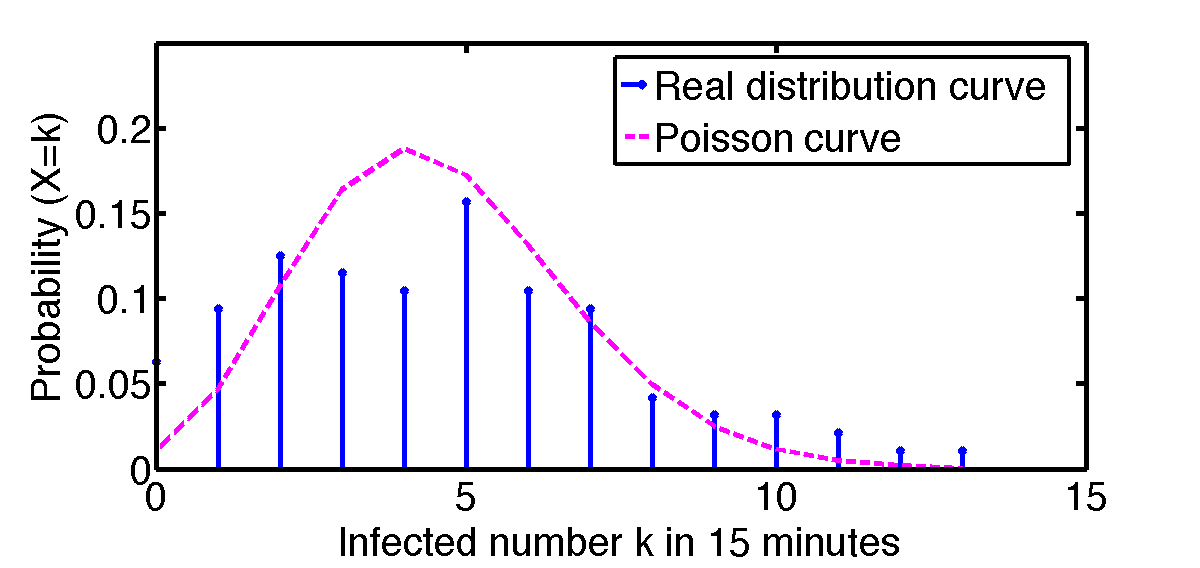
\includegraphics[width=3in,height=1.5in] {figures/poissonianCurve.png}
  \label{fig:poissonianCurve}
 }
\caption{Poisson distribution in latent space propagation. (a) shows the raw data outside of the mentions network of teacher protest events on Sept 3, 2013. (b) shows the probability distribution of the number of
infections.}
\label{fig:Poisson}
\end{figure}






\begin{table*}[t]
\label{table:massprotests}
\caption{Mass protests studied in this chapter.}
\centering
\tiny
%\begin{tabular}{p{0.05\linewidth}p{0.25\linewidth}p{0.20\linewidth}p{0.05\linewidth}p{0.05\linewidth}p{0.05\linewidth}}
\begin{tabular}{lp{0.25\textwidth}p{0.25\linewidth}lll}
\hline \\
No. & Event & Hashtags & Country & Affected cities & Event date(s) \\
\hline \\
1. & YoSoy132 student movement & \#LaMarchaYoSoy132, \#YoSoy132, \#132, \#soy132 & Mexico & Nationwide & 2012-05-17 to 2012-05-25 \\ \\
2. & Anti-government protests against tax reform and other policies pursued by President Juan Manuel Santos & \#CacerolazoPaSantos, \#5D & Colombia & Nationwide & 2012-12-05 \\ \\
3. & Education reform protests by teachers& \#ReformaEducativa & Mexico & Nationwide & 2013-09-01  \\ \\
4. & Social protests against violence and crime  &	\#UruguayosIndignados, \mbox{\#HartosDeLaViolencia} & Uruguay & Montevideo & 2012-05-14 \\ \\
5. & Protests against the ``media law'' & \#LorenzettiNoMeFalles, \#MediosBuitres & Argentina & Buenos Aires & 2012-11-27 \\ \\
6. & Protests against Senate President Renan Calheiros's election & \#STFjulgueRenan, \mbox{\#SocorroJoaquim}, \#ForaRenan & Brazil & Nationwide& 2013-02-22 to 2013-02-26 \\ \\
7. & Anti-government student protests against abuse of public media for election campaign  & \#ConatelCareTabla & Venezuela & Caracas & 2013-03-20 \\[1ex]
\hline
\end{tabular}
\end{table*}




With the observed network further split into several communities, each community is intended to have its own model parameters for GBM. In GBM, $ln(S_t^{ij})$
is a Gaussian distribution $\mathcal{N}((\mu - \frac{\sigma^2}{2})t, \sigma ^{2}t)$. We assume that each user within a community shares the same $\mu$ and $\sigma$ so that each community has its characteristic $\mu$ and $\sigma$. As information propagates through the mentions network, it may pass through different communities.
For an infected user $v_i$ and one of the non-infected
neighbors $v_j \in N(v_i)$, we assume the following propagation
strategy:
\begin{itemize}
    \item If $v_i$ and $v_j$ are in the same community $c_i$, the propagation process will follow $\mathcal{B}_{c_i}(\mu_{c_i}, \sigma_{c_i}^2)$.
        %In this case, we consider the rest of the mention network as part of that user's community, ${c_i}$.
    \item Propagation from one community to another happens as per the source community's model parameters. For instance, for propagation from community ${c_i}$ to community ${c_j}$, we will use the source community ${c_i}$'s GBM parameters.
    \item After information propagates into a different community, it will spread according to the new community's parameters. Once the information has entered community ${c_j}$ from community ${c_i}$, subsequent infections henceforth
will use community ${c_j}$'s parameters.
\end{itemize}

\noindent
At each time step we use the $\mu$ and $\sigma$ of any given node's current community for propagation from that node.
\subsection{Propagation in Latent Space}
As mentioned before, in the latent space, we are modeling unobserved interactions of users. Since there are so many factors that might affect the dissemination of information, such as news outlets, word-of-mouth, it is reasonable to assume that the probability of the number of newly infected users in a given time interval satisfies the Poisson distribution~\cite{haight1967handbook} in the latent space.

For each node in the mentions network, it can only be infected by the GBM process. However, for those isolated users outside the mentions network, it is only possible that they get infected via the mechanics of the Poisson process.
(Recall that in the GBM process, users get infected primarily
via their neighbors.) We use $X$ to represent the number of infected users
with time interval $\delta t$ and so the probability of the infected users is
given by:
\begin{equation}\Pr(X=k)= \frac{\lambda^k e^{-\lambda}}{k!}\end{equation}
To obtain an estimator of $\lambda$, we can only use information
about Twitter users who are outside the mentions network as our training dataset. We count the infected users outside the mentions network with time interval of 15 minutes during the Mexican teachers protest, and plot them as shown in Fig.~\ref{fig:Poisson_Sep3}.
Adequately modelable by a Poisson distribution, we use the average value as the estimate of $\lambda$. Fig.~\ref{fig:poissonianCurve} depicts the Poisson distribution fit with $\hat{\lambda}=4.18$. If there are $M_0$ isolated users, the probability of each of these users to get infected in time interval $\delta t$ is $\lambda/M_0$.
To summarize, for any user not in the mentions network, infection
is only possible via the Poisson process. For a user who is already in the
mentions network, infection can only happen via the GBM process over the mentions network, as described earlier.
